\section{Introduction}
%Most of the work is still in preparing the data
%Data preparation is done manually - either by writing a program or using data manipulation software (Excel)
While the quality and ease of use of data mining libraries such as in R~\cite{R2008} and Weka~\cite{Hall2009} is excellent, users must spend significant effort to prepare raw data for use in these libraries. In practice, the data preparation task is separate from the data mining process and very often requires data source dependent and repetitive manual work, such as applying Structured Query Language (SQL) statements to extract and aggregate database records, using Microsoft Excel to clean and normalize datasets of structured text files, and writing scripts to apply complex transformations (e.g., in Python). This practice does not scale when the data size becomes larger and the number of data sources increases.

In a previous work, Knoblock et al.~\cite{knoblock11:lisc,knoblock12:eswc} developed an interactive approach to extracting, modeling, and publishing data in a system called Karma.\footnote{See http://www.isi.edu/integration/karma for a video demonstration and details on Karma. The software is available as open source (Apache 2 License).} Karma allows an end-user to solve their own integration tasks without having to program those tasks. Karma can semi-automatically build a semantic description (a model) of a data source. This semantic description makes it possible to rapidly convert a set of sources (represented in Extensible Markup Language (XML), Javascript Object Notation (JSON), structured text files, or databases) into a shared domain model, which supports the integrated reasoning and processing of data across many sources. Once a user models the data sources, Karma can automatically converts the raw data into any of a variety of formats.

In this paper we present an integrated approach built on Karma for information integration and data mining. Our approach combines the steps in data preparation and data mining into a single integrated process and maintains detailed metadata about the data sources. We show that a user can use our approach to rapidly clean, normalize, restructure, integrate data collected from multiple mobile sensors, and then apply machine learning algorithms from a library of algorithms to perform a data mining task. We demonstrate these capabilities using a data mining task of predicting the mode of transport of a user given the sensor data collected via his/her cellphone. The challenge here is how to perform a data mining task, such that there is an sizable reduction in overall user time and effort in preparing the data set from its raw form and invoking the prediction service. We compare our approach with a baseline approach that uses Microsoft Excel for most of the data preparation tasks. We show how Karma supports the required steps for data preparation and data mining, and yields a significant reduction in time and effort.

The remainder of this paper is organized as follows. Section~2 describes a motivating data mining problem on prediction of mode of transport from mobile sensor data. Section~3 presents our integrated approach to data preparation and data mining. Section~4 describes the steps of using Excel to prepare raw data for data mining. Section~5 reports on our experimental results. Section~6 discusses the related work, and Section~7 presents discussion and future work.

\begin{figure}[ht!]
\centering
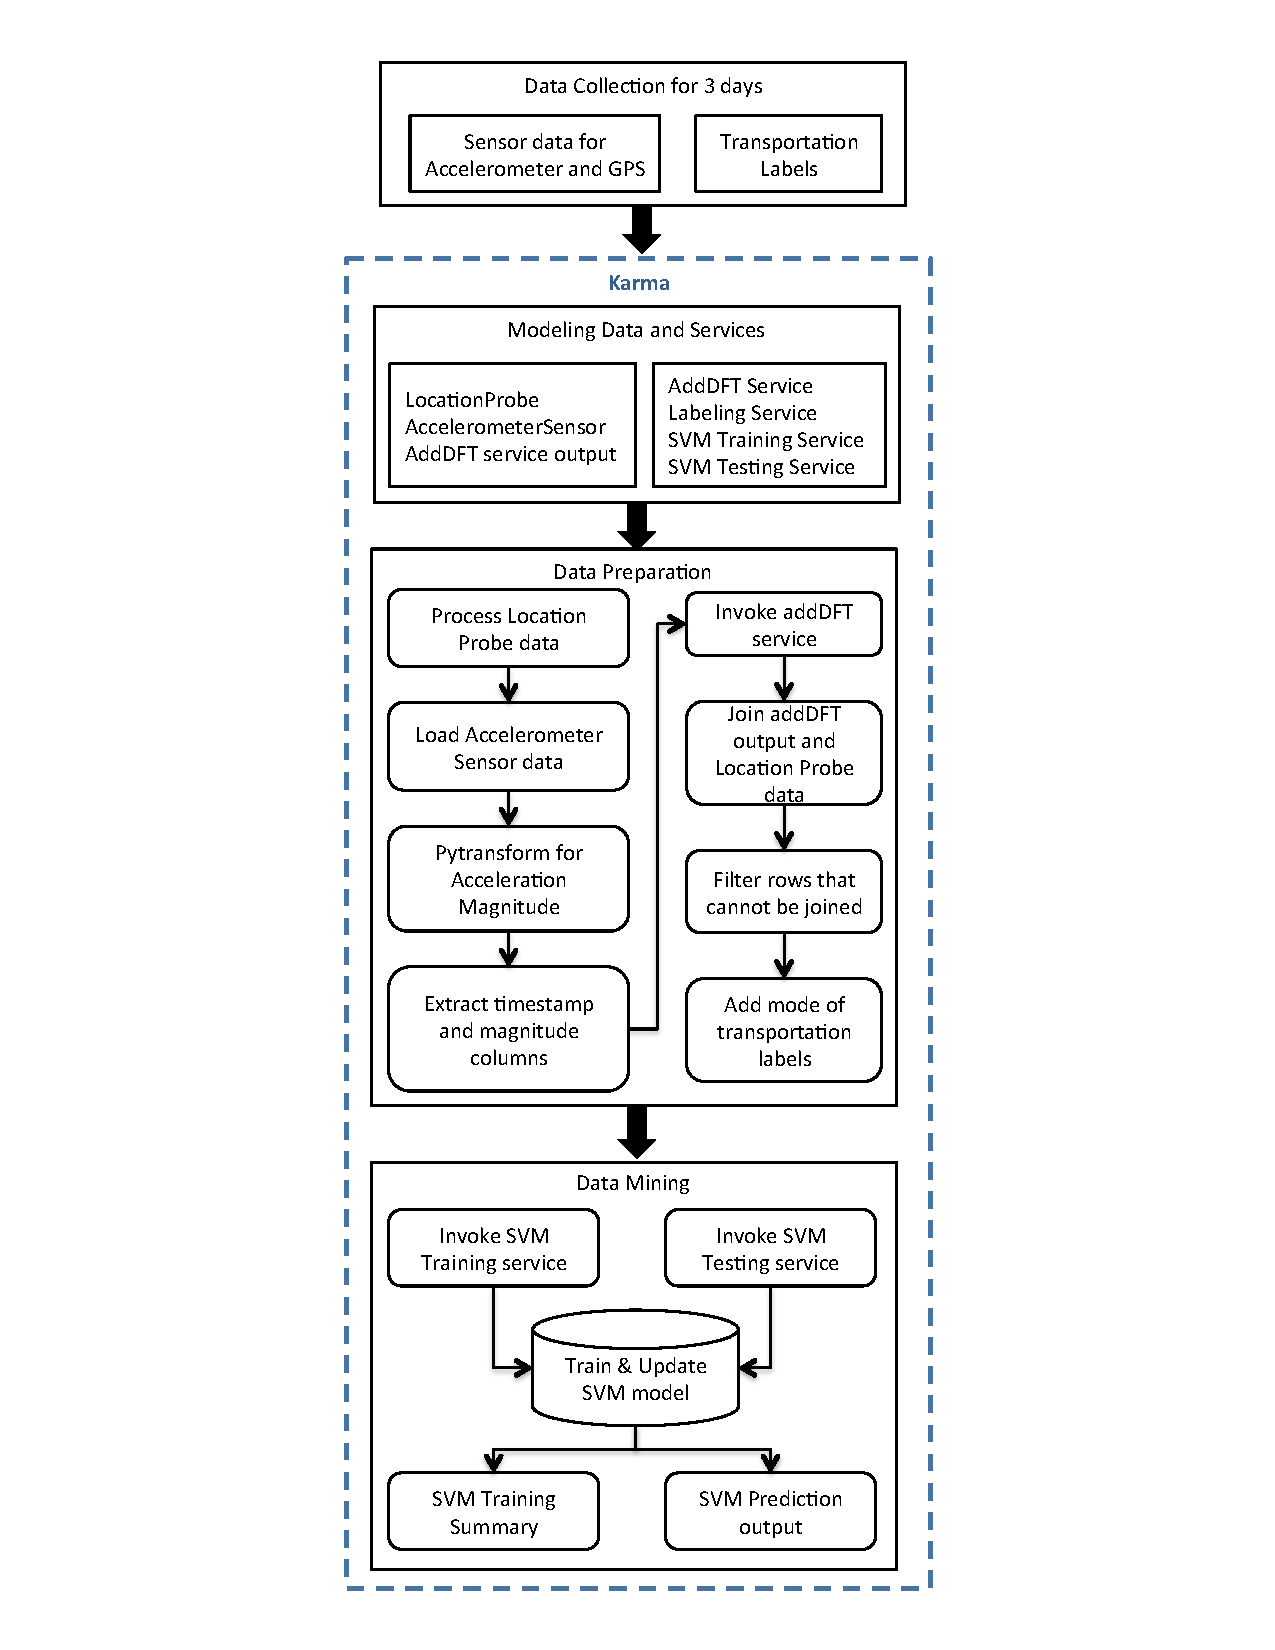
\includegraphics[width=80mm]{img/system_diagram.pdf}
\caption{System block diagram\label{fig:system_diagram}}
\end{figure}